\newpage

\section{Numerical Differentiation \& Numerical Integration}

Consider the problem of computing the integral
\begin{equation}
    I = \int_{1}^{2} \ln(f''(x)) \, dx,
\end{equation}
where smooth function $f$ is not known but its values over the interval $[1, 2]$ are given in the following table:

\begin{center}
\resizebox{\textwidth}{!}{
\begin{tabular}{|c|*{11}{c|}}
\hline
$x_k$ & 1 & 1.1 & 1.2 & 1.3 & 1.4 & 1.5 & 1.6 & 1.7 & 1.8 & 1.9 & 2 \\
\hline
$f(x_k)$ & 0.4 & 0.752 & 1.236 & 1.864 & 2.648 & 3.6 & 4.732 & 6.056 & 7.584 & 9.328 & 11.3 \\
\hline
\end{tabular}
}
\end{center}  

\vspace{10pt}
\subsection{Solution \& Results}

\subsubsection{Calculation of the Second Derivative}

To calculate the second derivative of discrete data, we use finite difference formulas. These formulas estimate the derivative at a specific point by using the function values at neighboring points. The constant distance between these points is called $h$. We must use three different formulas to process the entire dataset.

\begin{enumerate}
    \item \textbf{Central Difference Formula} \cite[page 329]{MathewsFink2003} \\
    For all points in the middle of our dataset, we use the central difference formula. This is the most standard method because it uses points on both the left and right sides of the target point.
    \begin{equation*}
        f''(x_i) \approx \frac{f_{x_{i-1}} - 2f_{x_{i}} + f_{x_{i+1}}}{h^2}
    \end{equation*}

    \item \textbf{Forward Difference Formula} \cite[page 333]{MathewsFink2003} \\
    For the very first point in our dataset, we cannot look backward because there are no previous points. Instead, we use a one-sided forward difference formula. This looks at the current point and the next three points ahead.
    \begin{equation*}
        f''(x_0) \approx \frac{2f_0 - 5f_1 + 4f_2 - f_3}{h^2}
    \end{equation*}

    \item \textbf{Backward Difference Formula} \cite[page 333]{MathewsFink2003} \\
    Similarly, for the very last point in the dataset, we cannot look forward. We use a one-sided backward difference formula. This looks at the current point and the three previous points behind it.
    \begin{equation*}
        f''(x_0) \approx \frac{2f_0 - 5f_{-1} + 4f_{-2} - f_{-3}}{h^2}
    \end{equation*}
\end{enumerate}

\vspace{5pt}
\noindent\textbf{Calculated second derivative vector:} \\
The calculations produced the following $11$ values (rounded for clarity):

\begin{center}
\resizebox{\textwidth}{!}{
\begin{tabular}{|c|*{11}{c|}}
\hline
$f''$ & 12 & 13.2 & 14.4 & 15.6 & 16.8 & 18 & 19.2 & 20.4 & 21.6 & 22.8 & 24 \\
\hline
\end{tabular}
}
\end{center}

\vspace{5pt}
\noindent\textbf{Natural logarithm of the second derivative vector ($\ln(f'')$):} \\
Next, we applied a natural logarithm to each element in the $f''$ vector, which produced the following values:

\begin{center}
\resizebox{\textwidth}{!}{
\begin{tabular}{|c|*{11}{c|}}
\hline
$\ln(f'')$ & 2.4849 & 2.5802 & 2.6672 & 2.7473 & 2.8214 & 2.8904 & 2.9549 & 3.0155 & 3.0727 & 3.1268 & 3.1781 \\
\hline
\end{tabular}
}
\end{center}

\vspace{10pt}
\subsubsection{Numerical Integration}

To calculate the definite integral from our discrete data points, we use numerical integration methods. 

\vspace{5pt}
\noindent\textbf{1. Trapezoidal Rule} \cite[page 255]{Sauer2014}

This method approximates the area under the function by connecting the data points with straight lines. This creates a series of trapezoids.

\begin{itemize}   
    \item \textbf{Formula:} To find the total area, we sum the areas of all the small trapezoids. The formula multiplies the endpoints by $1$ and all the middle points by $2$:
    \begin{equation}
        T(f, h) = \frac{h}{2}(f_0 + 2f_1 + 2f_2 + \dots + 2f_{M-1} + f_M)
    \end{equation}
    
    \item \textbf{Order of convergence:} The Trapezoidal Rule has a theoretical order of convergence of $2$, meaning the global error is proportional to $h^2$.
    
    \item \textbf{Result:} Applying this rule to our previously calculated data vector ($\ln(f'')$), the code produced the following integral value:
    \begin{equation*}
        \text{Trapezoidal Sum} = 2.870784586533755
    \end{equation*}
\end{itemize}

\vspace{5pt}
\noindent\textbf{2. Simpson's Rule} \cite[page 257]{Sauer2014}

Instead of straight lines, this method uses parabolas (quadratic curves) to connect sets of three adjacent points. This provides a much smoother fit to the data.

\begin{itemize}    
    \item \textbf{Formula:} This method requires an even number of subintervals ($2M$). The formula uses an alternating pattern of $4$ and $2$ for the middle points:
    \begin{equation}
        S(f, h) = \frac{h}{3}(f_0 + 4f_1 + 2f_2 + 4f_3 + \dots + 2f_{2M-2} + 4f_{2M-1} + f_{2M})
    \end{equation}
    
    \item \textbf{Order of convergence:} Simpson's Rule has a theoretical order of convergence of $4$, meaning the global error is proportional to $h^4$.
    
    \item \textbf{Result:} Applying Simpson's Rule to our data vector ($\ln(f'')$), the code produced the following integral value:
    \begin{equation*}
        \text{Simpson Sum} = 2.871200053592807
    \end{equation*}
\end{itemize}

\vspace{10pt}
\subsubsection{Error Analysis and Comparison}

To check the accuracy of our numerical methods, we compared our calculated sums to the exact given mathematical result.

\vspace{5pt}
\noindent\textbf{1. Exact Value and Calculated Errors} \\
The exact value of the integral is $2.871201010907891$. \\
By calculating the difference between this exact value and our numerical sums, we found the absolute error for each method:
\begin{itemize}
    \item \textbf{Trapezoidal Error (\texttt{trap\_err}):} $4.164243741358042 \times 10^{-4}$
    \item \textbf{Simpson's Error (\texttt{simp\_err}):} $9.573150840935796 \times 10^{-7}$
\end{itemize}

\vspace{5pt}
\noindent\textbf{2. Comparison of Errors} \\
When we compare the two errors, it is clear that Simpson's Rule is much more accurate. The error for the Trapezoidal Rule is around $4.16 \times 10^{-4}$, while the error for Simpson's Rule is much smaller, around $9.57 \times 10^{-7}$. This means that the error from Simpson's Rule is hundreds of times smaller than the error from the Trapezoidal Rule.

\vspace{5pt}
\noindent\textbf{3. Explanation} \\
We can explain this large difference in accuracy by looking at how each method works mathematically.
\begin{itemize}
    \item \textbf{Trapezoidal Rule} connects points with straight lines. It has an order of convergence of $2$. Usually used when points are not evenly distributed or the number of subintervals is odd (number of points is even).
    \item \textbf{Simpson's Rule} connects points using curved parabolas. It has a higher order of convergence of $4$. Requires an odd number of points. Usually used for evenly distributed points. 
\end{itemize}

Since the best conditions for Simpson's are met (odd number of evenly distributed points) and it has a higher order, its error shrinks much faster, giving much better results.

\subsection{Conclusions}

Based on the calculations and error analysis performed in this section, we can draw the following conclusions:

\begin{itemize}
    \item \textbf{Comparison of integration methods:} Both the Trapezoidal Rule and Simpson's Rule provided good approximations of the true integral area. However, their levels of accuracy were very different.
    
    \item \textbf{Advantage of Simpson's Rule:} The error analysis proved that Simpson's Rule ($9.57 \times 10^{-7}$) was significantly more accurate than the Trapezoidal Rule ($4.16 \times 10^{-4}$).
    
    \item \textbf{Reasons for different accuracy:} This difference in accuracy is expected based on the mathematical theory. Because our dataset had an odd number of evenly spaced points ($11$ points, $10$ subintervals), it was the perfect setup for Simpson's Rule. Since Simpson's Rule uses curved parabolas (O($h^4$) error) rather than the straight lines of the Trapezoidal Rule (O($h^2$) error), it fits the data much better and produces a much smaller error.
\end{itemize}

\newpage


\section{Interpolation \& Curve Fitting}

The concentration of \textit{E. coli} bacteria in a swimming area was measured after a storm and the data is given in the following table.

\begin{table}[h!]
    \centering
    \begin{tabular}{cc}
        Time $t$ (hours) & Concentration $c$ (CFU/100 mL) \\
        4  & 1600 \\
        8  & 1320 \\
        12 & 1000 \\
        16 & 890  \\
        20 & 650  \\
        24 & 560  \\
    \end{tabular}
\end{table}

Consider the problem of estimating the concentration of \textit{E. coli} bacteria at the end of the storm, i.e. at time $t = 0$.  

\subsection{Solution \& Results}

\subsubsection{Theory of Newton Polynomial Interpolation}

Newton Interpolation Method is a way to construct a mathematical curve that passes exactly through a specific set of data points. If we have $N + 1$ distinct data points, this method creates a unique polynomial of degree $N$ or less.

To build this polynomial, we use a mathematical tool called divided differences.

\vspace{5pt}
\noindent\textbf{1. Divided Differences} \cite[page 223]{MathewsFink2003} \\
Divided differences are calculated step-by-step from our given data points $(x_k, y_k)$.
Zeroth-order difference is simply the function value at that point:
\begin{equation*}
    f[x_k] = f(x_k)
\end{equation*}

The first-order difference uses two neighboring points:
\begin{equation*}
    f[x_{k-1}, x_k] = \frac{f[x_k] - f[x_{k-1}]}{x_k - x_{k-1}}
\end{equation*}

For higher orders, we use a recursive rule. We subtract two lower-order differences and divide by the total distance between the outermost $x$ values:
\begin{equation*}
    f[x_{k-j}, \dots, x_k] = \frac{f[x_{k-j+1}, \dots, x_k] - f[x_{k-j}, \dots, x_{k-1}]}{x_k - x_{k-j}}
\end{equation*}

\vspace{5pt}
\noindent\textbf{2. Divided-Difference Table} \cite[page 224]{MathewsFink2003} \\
In practice, these calculations are organized into a table. The first two columns contain the given $x$ and $f(x)$ values. Each new column to the right calculates the next level of divided differences using the values from the column before it. The most important numbers in this table are the ones located on the main diagonal.

\vspace{5pt}
\noindent\textbf{3. The Newton Polynomial Formula} \cite[page 220 - 221]{MathewsFink2003} \\
Once the table is complete, we can write the final polynomial. The Newton form of the polynomial is written as:
\begin{equation}
    P_N(x) = a_0 + a_1(x - x_0) + a_2(x - x_0)(x - x_1) + \dots + a_N(x - x_0)(x - x_1)\dots(x - x_{N-1})
\end{equation}
The coefficients ($a_0, a_1, \dots, a_N$) are the diagonal entries from our divided-difference table.

\vspace{5pt}
\subsubsection{Application of Newton Interpolation Method}
\noindent\textbf{1. Divided Differences Matrix $A$} \\
Based on input $t$ and $c$ values we can construct the Divided Differences table (lower triangular matrix):
\begin{equation*}
    A = \begin{bmatrix} 
        1600 & 0 & 0 & 0 & 0 & 0 \\ 
        1320 & -70 & 0 & 0 & 0 & 0 \\ 
        1000 & -80 & -1.25 & 0 & 0 & 0 \\ 
        890 & -27.5 & 6.5625 & 0.6510 & 0 & 0 \\ 
        650 & -60 & -4.0625 & -0.8854 & -0.0960 & 0 \\ 
        560 & -22.5 & 4.6875 & 0.7292 & 0.1009 & 0.0098 
    \end{bmatrix}
\end{equation*}

\vspace{5pt}
\noindent\textbf{Coefficient Vector $p$} \\
The coefficients of Newton polynomial correspond to the diagonal elements of matrix $A$. The decimal values:
\begin{equation*}
    p = \begin{bmatrix} 
        1600 \\ -70 \\ -1.25 \\ 0.6510416667 \\ -0.0960286458 \\ 0.0098470052 
    \end{bmatrix}
\end{equation*}

\vspace{5pt}
\noindent\textbf{Interpolation Nodes} \\
\begin{equation*}
    t = \begin{bmatrix} 4 & 8 & 12 & 16 & 20 & 24 \end{bmatrix}
\end{equation*}

\vspace{5pt}
\noindent\textbf{2. Construction of the Newton Polynomial} \\
The formula of the Newton interpolation polynomial for the given nodes has the following form:
\begin{equation*}
    P(t) = p_0 + p_1(t - t_0) + p_2(t - t_0)(t - t_1) + \dots + p_n(t - t_0)\dots(t - t_{n-1})
\end{equation*}
Tuning in values of the nodes $t_i$ and the decimal coefficients $p_i$, we obtain following polynomial:
\begin{equation}
    \begin{aligned}
        P(x) ={}& 1600 - 70(x - 4) - 1.25(x - 4)(x - 8) \\
        &+ 0.6510416667(x - 4)(x - 8)(x - 12) \\
        &- 0.0960286458(x - 4)(x - 8)(x - 12)(x - 16) \\
        &+ 0.0098470052(x - 4)(x - 8)(x - 12)(x - 16)(x - 20)
    \end{aligned}
\end{equation}

\vspace{5pt}
\noindent\textbf{3. Normalized Form of the Polynomial} \\
To reduce our polynomial to the classic form $P(x) = a_n x^n + a_{n-1} x^{n-1} + \dots + a_0$, the brackets are expanded and terms are grouped together.

\noindent Result in decimal form:
\begin{equation}
    \begin{aligned}
        P(x) ={}& 0.0098470052x^5 - 0.6868489583x^4 + 17.8841145833x^3 \\
        &- 212.4479166667x^2 + 1057.5833333333x - 210
    \end{aligned}
\end{equation}

\subsubsection{Graphical Analysis and the Limits of Extrapolation}

\begin{figure}[h]
    \centering
    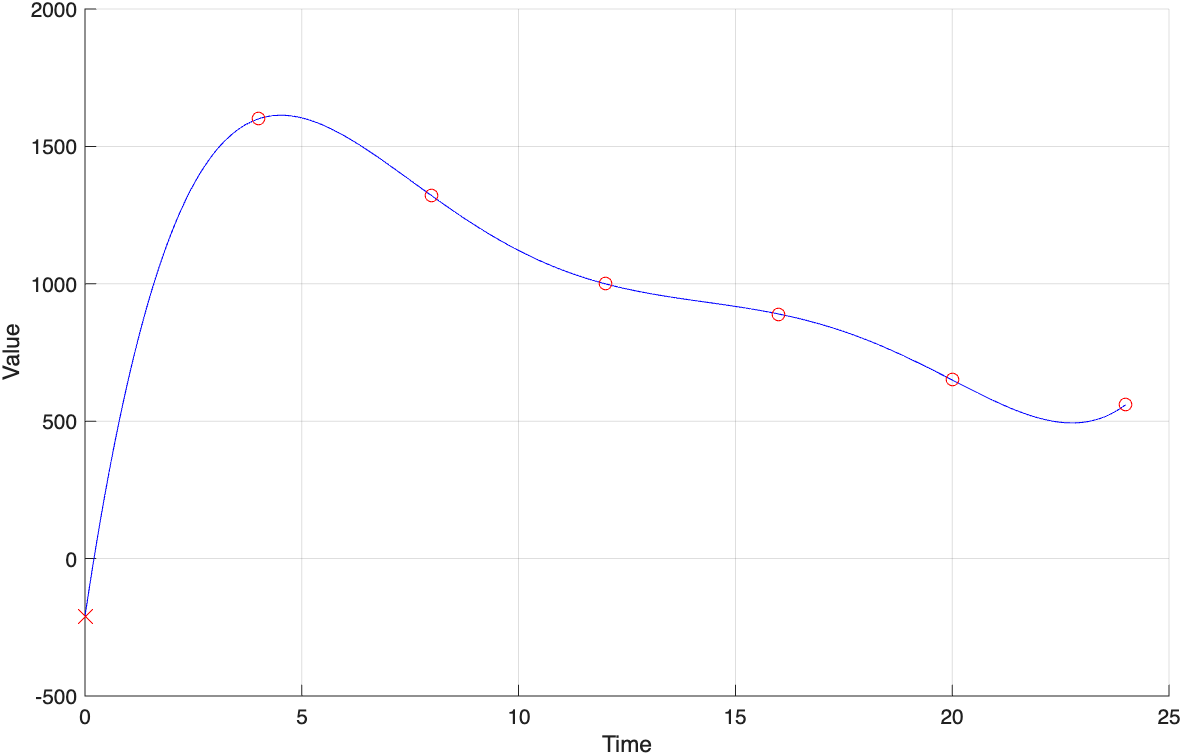
\includegraphics[width=1 \textwidth]{img/3_a_plot}
    \caption{Graph of obtained polynomial in the interval [0, 24] and the data points marked as circles where $t = 0$ (extrapolation point) marked as X-mark}
\end{figure}

\vspace{5pt}
\noindent\textbf{1. Interpolation Results} \\
The generated graph illustrates a 5th-degree polynomial curve (in blue) fitted to the discrete measurements of bacteria concentration over time. Within the bounds of our experimental data (from hour $4$ to hour $24$), the polynomial successfully acts as an interpolant. The curve captures a physically realistic trend during this timeframe: an initial spike in contamination following the storm, followed by a gradual decay as the system begins to clear.

\vspace{5pt}
\noindent\textbf{2. Polynomial Extrapolation} \\
Extrapolation involves utilizing our mathematical model to predict values outside the domain of the measured data (specifically, before hour $4$ and after hour $24$). When evaluating the polynomial at $x = 0$, the model yields a concentration of $-210$.

\vspace{5pt}
\noindent This negative result occurs for two primary reasons:
\begin{itemize}
    \item \textbf{Mathematical Limitations:} High-degree polynomials (like our 5th-degree model) are unstable outside their interpolation interval. They tend to oscillate wildly once they pass the initial data points. The algorithm's objective was to minimize the error between the known data points, not to understand the broader context of the function.
    
    \item \textbf{Physical Impossibility:} In a real-world biological system, concentration cannot drop below zero. The mathematical model is purely algebraic and is unaware of physical boundary conditions unless they are specifically programmed into it.
\end{itemize}

\subsubsection{Theory of Least-Squares Fitting}

Curve fitting is a mathematical process used to construct a continuous function that best represents a set of discrete data points. Unlike interpolation (which forces the curve to pass exactly through every point), the least-squares method finds a "best fit" model by minimizing the overall error (in this case RMS) between the calculated curve and the actual data.

\vspace{5pt}
\noindent\textbf{1. Linear Curve Fitting (The Least-Squares Line)} \cite[page 255]{MathewsFink2003} \\
If we have a dataset of $N$ distinct points $(x_k, y_k)$, the simplest approach is to fit a straight line. The equation for this line is:
\begin{equation*}
    y = Ax + B
\end{equation*}
To find the optimal coefficients $A$ (the slope) and $B$ (the y-intercept) that minimize the error, we must solve a specific linear system known as the normal equations. By summing the combinations of our data points, we set up the following two equations:
\begin{align*}
    \left(\sum_{k=1}^N x_k^2\right)A + \left(\sum_{k=1}^N x_k\right)B &= \sum_{k=1}^N x_k y_k \\
    \left(\sum_{k=1}^N x_k\right)A + N B &= \sum_{k=1}^N y_k
\end{align*}
Solving this system simultaneously provides the exact values for $A$ and $B$ to construct the best-fit line.

\vspace{5pt}
\noindent\textbf{2. Exponential Curve Fitting (Data Linearization)} \cite[page 263]{MathewsFink2003} \\
Often, physical processes (like bacterial decay or population growth) do not follow a straight line and are better modeled by an exponential curve:
\begin{equation*}
    y = Ce^{Ax}
\end{equation*}
Because this equation is non-linear, we cannot apply the normal equations directly. Instead, we must use a technique called data linearization.

\vspace{5pt}
\noindent\textbf{Step 1: Logarithmic Transformation} \\
We take the natural logarithm of both sides of the equation to break down the exponential term:
\begin{equation*}
    \ln(y) = Ax + \ln(C)
\end{equation*}

\vspace{5pt}
\noindent\textbf{Step 2: Change of Variables} \\
We introduce new variables to rewrite the equation in a standard linear format. Let:
\begin{align*}
    Y &= \ln(y) \\
    X &= x \\
    B &= \ln(C)
\end{align*}
This transforms our complex equation into a simple linear relation:
\begin{equation*}
    Y = AX + B
\end{equation*}

\vspace{5pt}
\noindent\textbf{Step 3: Applying the Normal Equations} \\
We map our original data points $(x_k, y_k)$ to the new linearized plane, creating transformed points $(X_k, Y_k) = (x_k, \ln(y_k))$. We then feed these $X$ and $Y$ values into the standard normal equations (from Part 1) to solve for $A$ and $B$.

\vspace{5pt}
\noindent\textbf{Step 4: Reversing the Transformation} \\
Once the linear system is solved, the parameter $A$ is ready to use. However, $B$ is still in its logarithmic form. To find the original coefficient $C$ for our exponential model, we compute the inverse logarithm:
\begin{equation*}
    C = e^B
\end{equation*}
This process allows us to accurately fit complex, non-linear curves using standard, reliable linear algebra tools.

\vspace{5pt}
\noindent\textbf{3. RMS} \cite[page 253]{MathewsFink2003} \\
The Root-Mean-Square error is a very common and useful way to find the overall error. To calculate it, you square every residual, find the average of all those squared values, and finally take the square root of that average.

The formula for the RMS error ($E$) for $N$ data points is:
\begin{equation}
    E(f) = \left( \frac{1}{N} \sum_{k=1}^{N} |f(x_k) - y_k|^2 \right)^{1/2}
\end{equation}

In curve fitting, the RMS error is often preferred because squaring the errors strongly penalizes points that are very far away from the curve.

\subsubsection{Results and Comparison of Curve Fitting Models}

\vspace{5pt}
\noindent\textbf{1. Calculation of Coefficients} \\
To create our models, we applied the least-squares theory using our MATLAB code. For the linear model, we directly passed the time and concentration arrays into our solver function to find the straight-line coefficients. For the exponential model, we first linearized the data by taking the natural logarithm of the concentration array ($\ln(c)$). We passed this modified data into the same solver. Then, we transformed the resulting parameter back into our final exponential constant by using the $\exp()$ function, exactly as described in the theory.

\vspace{5pt}
\noindent\textbf{2. Graphical and Numerical Results} \\

\begin{figure}[h]
    \centering
    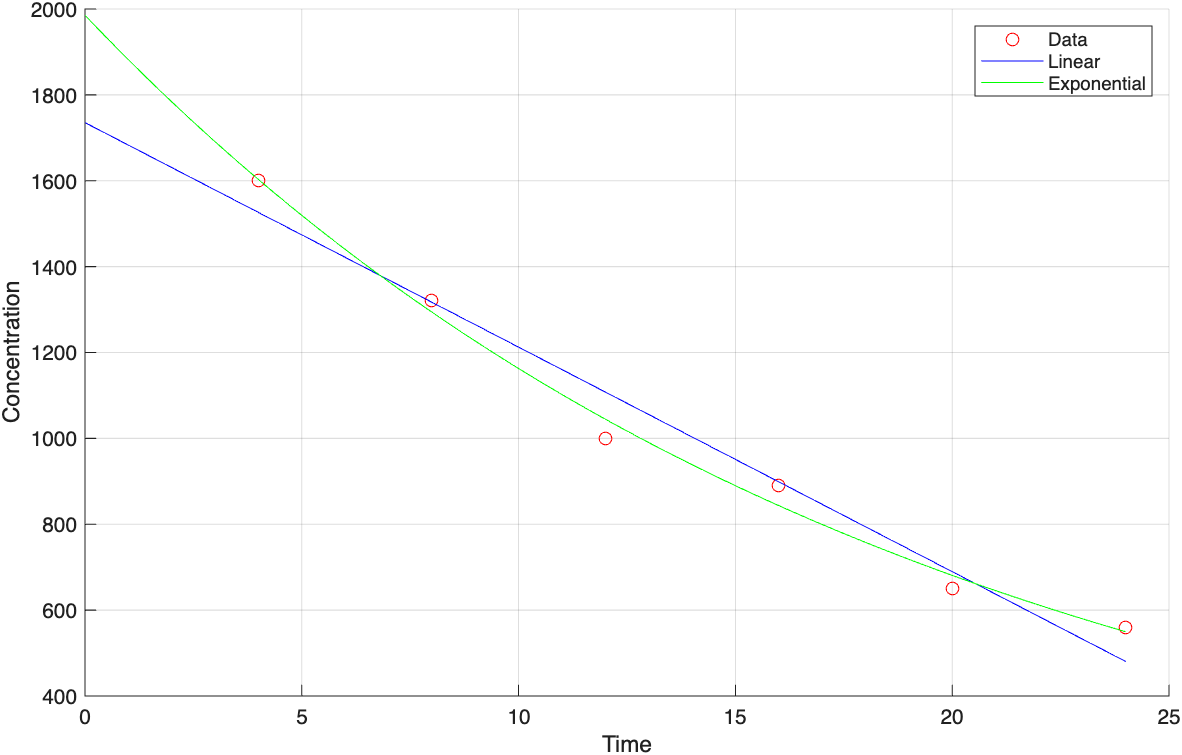
\includegraphics[width=1 \textwidth]{img/3_d_plot}
    \caption{Resulting least squares line, the least squares exponential curve and the given data points}
\end{figure}

We used both models to extrapolate backward to $t=0$. This gives us an estimate of the bacteria concentration at the exact moment the storm happened. We also calculated the Root Mean Square (RMS) error. This number tells us how far off our calculated line is from the real data points (a lower number is better).

The program gave these results:
\begin{itemize}
    \item \textbf{Linear Model:} The estimated concentration at $t=0$ is $1735.33$. The RMS error is $64.64$.
    \item \textbf{Exponential Model:} The estimated concentration at $t=0$ is $1985.44$. The RMS error is $31.39$.
\end{itemize}

\vspace{5pt}
\noindent\textbf{3. Comparison} \\
When we compare two methods, exponential model is clearly superior to linear.

\begin{itemize}
    \item \textbf{Error Analysis:} The RMS error for the exponential curve ($31.39$) is more than two times smaller than the error for the straight line ($64.64$). This proves the green curve fits our dataset much better mathematically.
    \item \textbf{Visual:} Looking at the graph, the blue straight line completely misses the middle points and the final point. The green curve naturally bends and passes very close to almost all the red circles.
    \item \textbf{Reality:} In biology, natural decay processes usually follow an exponential curve. When there is a lot of bacteria, the concentration drops quickly. As the water gets cleaner, the rate of decay slows down. The linear model is flawed because it assumes the bacteria disappear at the exact same constant speed forever.
\end{itemize}


\subsection{Conclusions}

Based on the analysis of the different mathematical models in this section, we can draw the following conclusions regarding the initial bacteria concentration:

\begin{itemize}
    \item \textbf{Failure of Polynomial extrapolation:} While the 5th-degree Newton polynomial perfectly connected our known data points, it completely failed at predicting the past. It produced an impossible negative concentration ($-210$) for time zero. This proves that high-degree polynomials are highly unstable and should not be used for extrapolation outside the given data range.

    \item \textbf{Inaccuracy of the Linear model:} The linear least-squares model assumed the bacteria died at a constant speed. This resulted in a poor fit with a high error ($\text{RMS} = 64.64$) because a straight line does not reflect how real biological decay works.

    \item \textbf{Superiority of the Exponential model:} The exponential model performed much better. It had an error that was more than two times smaller ($\text{RMS} = 31.39$) and correctly matched the natural biological process, where the rate of bacterial decay naturally slows down as the water gets cleaner.

    \item \textbf{Final Estimation:} Because the exponential curve is the most mathematically accurate and physically realistic model for this dataset, we conclude that our best estimate for the initial \textit{E. coli} concentration right after the storm is $1985.44$ CFU/100 mL.
\end{itemize}